\documentclass[10pt,journal]{IEEEtran}

\usepackage{amsmath,amssymb}
\usepackage{array}
\usepackage{booktabs}
\usepackage{float}
\usepackage{graphicx}
\usepackage{microtype}
\usepackage{multirow}
\usepackage{url}
\usepackage{xcolor}
\usepackage{tikz}
\usetikzlibrary{arrows.meta,fit,positioning}

\definecolor{accentblue}{HTML}{24557A}
\definecolor{accentteal}{HTML}{2A7F78}
\definecolor{accentorange}{HTML}{C56A2D}
\definecolor{softblue}{HTML}{EAF1F7}
\definecolor{softgray}{HTML}{F2F3F5}
\definecolor{passgreen}{HTML}{26734D}
\definecolor{failred}{HTML}{A23B3B}

\newcommand{\method}{calibrated expected-F1}
\newcommand{\pass}{\textcolor{passgreen}{\textbf{Pass}}}
\newcommand{\fail}{\textcolor{failred}{\textbf{Fail}}}
\newcommand{\theadrow}{}
\graphicspath{{figures/}}
\interdisplaylinepenalty=2500
\hyphenation{multi-modal fact-check-ing re-triev-al cal-i-bra-tion}

\title{Retrieval-Conditioned Calibration and Adaptive Evidence Selection for Multimodal Fact-Checking}

\author{%
\parbox[t]{0.46\textwidth}{\centering
Sabbir Hossain\\[0.3ex]
{\normalsize
Department of Computer Science\\
American International University-Bangladesh\\
Dhaka, Bangladesh\\
26-94030-1@student.aiub.edu}}
\hspace{0.02\textwidth}%
\parbox[t]{0.46\textwidth}{\centering
Dr.~Firoz Ahmed\\[0.3ex]
{\normalsize
Professor, Faculty\\
Department of Computer Science\\
American International University-Bangladesh\\
Dhaka, Bangladesh\\
fahmed@aiub.edu}}}

\begin{document}
\maketitle

\begin{abstract}
However, it is impossible for an evidence selector to retrieve things that were not retrieved, and evidence selection based on probability is unreliable if the membership scores are not calibrated. We assess these coupled failures on MOCHEG and based on an organizer-store protocol that is separately frozen in AVerImaTeC. Label-blind rank fusion achieves F1 score of 0.3637 on MOCHEG compared to 0.3560 without it, and prior-aware calibration achieves mean Brier score of around 0.033 compared to 0.0847 without it. Calibrated thresholding is 0.1864 evidence F1, expected-F1 is 0.1815 with 3.61 instead of 5.26 items. The completeness-aware switch is at 0.1877, while the effect of its $+0.00138$ is not clear. Frozen packet has only 25.48\% exact annotated sources and 59.87\% of claims have no reachable target when it comes to locked AVerImaTeC development. Calibration transfers: the actual difference between a calibrated expected-F1 and an uncalibrated ablation is 0.0532 F1 and the multiplicity-adjusted interval is $[0.0221,0.0885]$. The other relationships fail: thresholding and fixed selection are tied, expected-F1 returns 3.20 items versus 1.17 for thresholding, the switch interval crosses zero after correction, and switch-selected evidence fails verifier non-inferiority. We do not have any local official semantic judge, and formal tests on both benchmarks have not been changed. The cross-benchmark evidence supports reachability-first, calibration-aware evaluation, but not adaptive-selector superiority or a universally compact expected-F1 policy.
\end{abstract}

\begin{IEEEkeywords}
multimodal fact-checking, evidence retrieval, evidence selection, probability calibration, expected F1, reproducibility
\end{IEEEkeywords}

\section{Introduction}
\label{sec:introduction}

An auditable fact-check exposes the evidence behind its verdict. For a multimodal claim, that evidence may include both passages and images from several sources. A retrieval system can supply hundreds of candidates, while a reviewer needs a manageable set that retains the material relevant to the decision. MOCHEG captures this setting with text and image evidence, released evidence identifiers, and three-way verdicts \cite{yao2023mocheg}.

A fixed top-$k$ rule returns a common evidence budget across claims. Adaptive policies can vary that budget. Thresholding selects items above a cutoff, a count model predicts the set size, and expected-$F_1$ decoding selects the probability-ranked prefix with the highest expected set $F_1$. A strictly increasing score transformation preserves rank while potentially changing threshold decisions and expected utility.

Evidence membership is sparse, and balancing the scorer's training data changes its effective class prior. This can introduce an intercept error in predicted log odds. Temperature scaling changes their slope, while a map with an intercept can also correct their offset. Assessing probability quality alongside ranking helps distinguish calibration effects from the behavior of the decoder \cite{silvafilho2023calibration}.

Retrieval forms an extra, more difficult boundary. Any item that does not make it into the packet cannot be returned by a selector. A decoding error and a retrieval miss will be given the same final evidence score if the packet reachability is not reported. The information boundaries followed here are shown in Figure~\ref{fig:architecture}. The same 40 text and 20 images candidates are given to all selection policies. The candidate rankings are recorded prior to the gold join, disjoint roles are used for scoring, calibration, policy selection and evaluation, and the released validation set is evaluated only after the train-role decisions have been made.

\begin{figure*}[t]
  \centering
  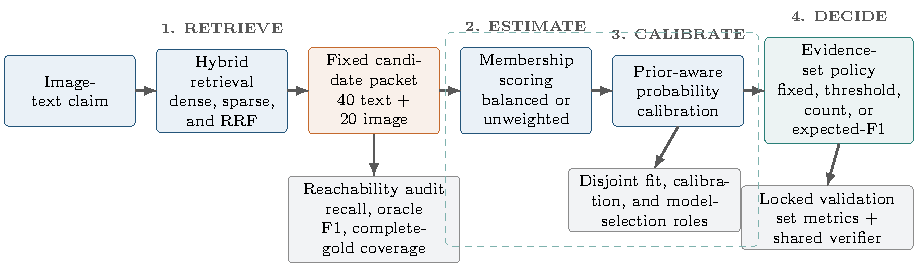
\includegraphics[width=\textwidth]{architecture.pdf}
  \caption{Study design and information boundaries. Label-blind retrieval fixes a candidate packet before gold identifiers are joined. Disjoint training roles support scoring, calibration, and policy selection. Locked validation compares matched evidence policies and a shared-verifier safeguard. Formal-test annotations remain outside the execution path}
  \label{fig:architecture}
\end{figure*}

We ask five questions.
\begin{enumerate}
    \item What is the amount of released gold evidence at the actual depths of the packets and can a ``bounded'' label-blind rank fusion increase that upper bound?
    \item Which calibration maps improve membership probabilities under class imbalance?
    \item What are the differences between fixed top-$k$, calibrated thresholding, learned count, expected-$F_1$ and an uncalibrated ablation on the same packets?
    \item Is a fixed ``packet completeness'' switch superior to calibrated thresholding and maintains a high level of verdict quality in the presence of a more powerful shared verifier?
    \item Which of these relationships reproduce under a separately frozen AVerImaTeC organizer-store protocol with different evidence units and four verdict classes?
\end{enumerate}

We compare candidate reachability, probability quality, evidence-set utility, and verdict performance under each benchmark's own protocol. Calibration improves the expected-$F_1$ ablation on both benchmarks. The compact operating point observed on MOCHEG reverses on AVerImaTeC, where expected-$F_1$ selects more sources than thresholding. This reversal illustrates why the decoder's tradeoff must be measured under the intended retrieval and scoring conditions.

This paper makes four contributions:
\begin{itemize}
    \item a retrieval-conditioned evaluation that reports the operating-depth recall, the packet-oracle $F_1$, the complete-gold coverage, and the zero-reachable claims before interpreting selector quality;
    \item a matched calibration and set-decoding study covering six probability maps, fixed and adaptive controls, exact expected-$F_1$, and an uncalibrated failure case;
    \item a prespecified retrieval repair and packet-completeness-aware switch, evaluated against the strongest calibrated-threshold comparator with claim-aligned intervals and partition-level safeguards; and
    \item an external evaluation on the organizer's static AVerImaTeC store, with train-only fitting, a frozen development comparison, and a post hoc audit of where exact targets are lost.
\end{itemize}

\section{Related Work}
\label{sec:related}

\begin{table*}[t]
\centering
\caption{Comparison with evidence-aware multimodal verification and retrieval studies. An output of a set of different sizes of evidence is called adaptive; reranking, filtering, and modality routing are not adaptive set decoding.}
\label{tab:related-comparison}
\small
\setlength{\tabcolsep}{4pt}
\renewcommand{\arraystretch}{1.13}
\begin{tabular}{@{}>{\raggedright\arraybackslash}p{0.12\textwidth}
>{\raggedright\arraybackslash}p{0.16\textwidth}
>{\raggedright\arraybackslash}p{0.28\textwidth}
>{\raggedright\arraybackslash}p{0.14\textwidth}
>{\raggedright\arraybackslash}p{0.17\textwidth}@{}}
\toprule
Study & Setting & Retrieval or selection mechanism & Set policy & Evaluated outputs \\
\midrule
MOCHEG \cite{yao2023mocheg} & Web fact-checking & Separate neural text and image retrieval & Fixed top-$k$ & Retrieval, verdict, explanation \\
RED-DOT \cite{papadopoulos2025reddot} & VERITE; NewsCLIPpings+ & Relevance detection and evidence reranking & Fixed pool with item masking & Item relevance, verdict \\
SciVer \cite{wang2025sciver} & Scientific papers & Foundation-model and RAG benchmark & No adaptive set policy & Evidence, verdict \\
MuSciClaims \cite{lal2025musciclaims} & Scientific figures & Figure localization and reasoning diagnostics & Provided figure context & Localization, verdict \\
M$^2$-TabFact \cite{zhou2025m2tabfact} & Multi-document tables & Textual and visual table evidence reasoning & Provided multimodal evidence & Verdict \\
MEVER \cite{zhang2026mever} & MOCHEG; FACTIFY; AIChartClaim & Graph retrieval and multimodal fusion & Fixed top-$k$ & Retrieval, verdict, explanation \\
Utility-oriented \cite{luo2026utility} & MRAG-Bench; Visual-RAG & Information-gain and helpfulness ranking & Fixed top-$K$ & Downstream answer utility \\
Selective retrieval \cite{tsoneva2026selective} & AVerImaTeC & Question-type routing with hybrid retrieval & Fixed per-question budget & Evidence, verdict, justification \\
\midrule
\textbf{This study} & \textbf{MOCHEG and AVerImaTeC organizer stores} & \textbf{Label-blind multimodal packets, calibrated membership scores, packet-completeness estimate} & \textbf{Fixed, threshold, expected-F1, and switch controls} & \textbf{Reachability, set F1, calibration, shared verifier, cross-benchmark transfer} \\
\bottomrule
\end{tabular}
\end{table*}

\subsection{Evidence-Based Fact-Checking and Evaluation}

Evidence-based verification can typically be broken down into four components: claim analysis, evidence retrieval, evidence assessment and verdict prediction \cite{zeng2021automated,zhou2020survey,islam2020survey}. The findings vary with the domain, label construction, modality coverage, and controls for event or source overlap, as documented in dataset surveys \cite{dulizia2021datasets,rastogi2022threet}. Difficulties with cross-domain transfer, deficient explanations, and benchmark protocols remain common \cite{mridha2021review,aimeur2023review,lv2025survey}. Our assessment therefore follows the retrieval-and-selection chain rather than content-only classification.

Evidence requirements are revealed through text benchmarks. SciFact contains sentence evidence from scientific publications, HoVer is multi-document reasoning, COVID-Fact is following evolving claims in the public-health arena, and X-Fact introduces multilingual variation \cite{wadden2020scifact,jiang2020hover,saakyan2021covidfact,gupta2021xfact}. External-document systems minimize reliance on stylistic shortcuts, while also incurring retrieval, freshness, and attribution errors \cite{zhang2023realtime}. So, we separate evidence-set quality and verdict accuracy.

\subsection{Multimodal Misinformation Detection}

Content-based multimodal detectors include bilinear pooling \cite{kumari2021amfb}, hierarchical attention \cite{meel2021han}, topic memory \cite{ying2021topicmemory} and cross-attention \cite{ying2021crossattention}, ambiguity learning \cite{chen2022cafe} and multi-level fusion \cite{jing2023mpfn} detectors. Contrastive, in-modality, stylometric or semantic-alignment signals are added in later systems \cite{yan2024fmc,zhu2024ifis,nadeem2023ssm,uppada2022imagetext}. These designs help to classify at the post level; however, the fused representation does not reveal the source of a verdict, such as an external document or image.

Recent works focus on local-global mismatch \cite{wu2023mfir}, cross-modal knowledge distillation \cite{hu2024matching,peng2024contextual}, contextual inconsistency \cite{shang2026semantic} and conflicting unimodal signals \cite{wang2024neutralization}. Out-of-context benchmarks like NewsCLIPpings \cite{luo2021newsclippings}, COSMOS \cite{aneja2023cosmos}, and VERITE \cite{papadopoulos2024verite} evaluate pairs of images and captions where they do not match in context but control unimodal bias. DGM4, SNIFFER, MMDFND, and IMFND extend localization, explanation, domain coverage or vision-language model usage \cite{shao2023dgm4,qi2024sniffer,tong2024mmdfnd,jiang2025imfnd}. They are not primarily aimed at a set of external evidence identifiers that can be audited, but at manipulation or veracity.

\subsection{Multimodal Evidence Retrieval and Verification}

MOCHEG offers a common evaluation criterion for multimodal retrieval, three-way verdict prediction and explanation generation \cite{yao2023mocheg}. MEVER builds a text--image evidence graph and performs token- and evidence-level fusion \cite{zhang2026mever}, while RED-DOT identifies and reranks external multimodal evidence before prediction \cite{papadopoulos2025reddot}. Other recent studies distinguish utility from semantic similarity and learn when visual retrieval is needed \cite{luo2026utility,tsoneva2026selective}. These systems address fixed retrieval, relevance filtering, modality routing, utility ranking, and adaptive set decoding as different decision problems.

AVerImaTeC assesses real-world image--text claims using open-web or organizer-provided knowledge, and its shared task conditions verdict scoring on evidence quality \cite{cao2026averimatecshared}. In that context, REVEAL combines iterative sparse and dense retrieval \cite{tariq2026reveal}. MOCHEG's stable item corpus differs from question--answer evidence and open-web access, so transfer requires a separately frozen unit definition and candidate-construction protocol.

\subsection{Scientific and Citation-Grounded Evidence}

Stable evidence locations in passages, tables and figures are provided by scientific verification. SciVer consists of claim-evidence instances extracted from scientific papers and annotated by experts; MuSciClaims focuses on figure-grounded claims and controlled reasoning perturbations; and M$^2$-TabFact covers tables presented across text and images \cite{wang2025sciver,lal2025musciclaims,zhou2025m2tabfact}. These tools can be used to make more precise localization analysis, but they do not explicitly reflect political or breaking-news verification.

An explanation might be expressed effectively, but with the use of the incorrect source. Evidence-rationale benchmarks check whether a prediction is connected to a selected span, and faithful-by-construction rationalizers limit predictors to explicit evidence subsets \cite{deyoung2020eraser,jain2020faithful}. Citation-grounded generation assesses whether retrieved sources support generated statements \cite{gao2023alce}; RAGTruth catalogs hallucinations that persist despite retrieval \cite{niu2024ragtruth}; and citation masking tests whether a fact-checking explanation recovers the correct evidence \cite{xing2025attribution}. The present study adopts released evidence identifiers rather than generated rationales and allows exact-set precision, recall, F1, Jaccard similarity and exact match.

\subsection{Calibration and Adaptive Set Decisions}

A score may rank a candidate correctly while remaining a poor probability. Post-hoc calibration includes temperature and Platt mappings, beta calibration, and nonparametric isotonic regression; each makes different assumptions about the distortion being corrected \cite{silvafilho2023calibration}. After class weighting, prior correction is important because the optimized training distribution differs from the operating distribution. The calibrated membership distribution can then support expected-utility decoding, while structurally different policies such as top-$k$, thresholding, and learned count use the same scores.

In this study, representation models and evidence identities remain fixed while a bounded, label-blind rank fusion changes only the retained ordering. The selector experiment then evaluates packet reachability, prior-aware probability correction, exact expected-F1 decoding, and one prespecified completeness-aware switch under matched candidates, tuning roles, and downstream verification. A separately frozen organizer-store run tests the same relationships on AVerImaTeC without transferring fitted MOCHEG parameters. This design isolates which conclusions are benchmark-specific and which survive a change in evidence units, candidate construction, and class balance (Table~\ref{tab:related-comparison}).

\section{Problem Definition and Data}
\label{sec:problem}

\subsection{Task}

Let claim $q$ have a released complete-gold evidence set $G_q$ and let retrieval return an ordered packet
\begin{equation}
C_q=(c_{q1},\ldots,c_{q60}),
\end{equation}
which can hold a maximum of 40 text candidates and 20 image candidates. A selector returns $S_q\subseteq C_q$. The main claim-level score is
\begin{equation}
F_1(S_q,G_q)=\frac{2|S_q\cap G_q|}{|S_q|+|G_q|}.
\label{eq:set-f1}
\end{equation}
We macro-average over claims in Eq.~\ref{eq:set-f1}. Other evidence metrics are precision, recall, Jaccard similarity, exact-set match and selected count.

The primary population includes only claims for which the released annotation defines a nonempty complete-gold set. Claims without such a mapping remain in retrieval construction and do not get a perfect oracle score. If they are given an oracle F1 of one, this will give the false impression of a high apparent packet ceiling.

\subsection{Dataset and Population Flow}

MOCHEG is a dataset that includes image-text claims, separate image and text evidence as well as verdict labels \cite{yao2023mocheg}. By content hash we pin released versions of the train, validation, corpus and sealed-test. The test annotations are not opened in the official test.

The 13,159 released train and validation claims are encoded for retrieval. Of these, 10,970 have a nonempty released complete-gold mapping and are the eligible evidence-set population. The primary repaired-packet selector evaluation uses the 1,490 released validation claims. Claim-grouped hashing places the remaining released claims in fitting, calibration, model-selection, and internal-holdout roles. The roles are regenerated separately for deterministic partition seeds 13, 37, 73, 101, and 137.

\begin{table}[t]
\centering
\caption{Evaluation population and reachable-evidence boundary.}
\label{tab:population-flow}
\begin{tabular}{lr}
\toprule
Population or boundary & Value \\
\midrule
Released train and validation claims & 13,159 \\
Claims with nonempty complete gold & 10,970 \\
Locked validation claims & 1,490 \\
Eligible claims with no reachable gold & 3,086 \\
Packet-oracle evidence F1 & 0.3560 \\
Complete-gold packet coverage & 4.39\% \\
\bottomrule
\end{tabular}
\end{table}


\subsection{Reachability}

The retrieval boundary is specified by two oracle summaries. For every eligible claim, the packet oracle returns $C_q\cap G_q$. Its F1 is averaged only for claims with nonempty gold. Complete-gold coverage is the fraction of eligible claims for which $G_q\subseteq C_q$ holds. We count eligible claims for which $C_q\cap G_q=\varnothing$.

These quantities provide answers to different questions. Oracle F1 is the best evidence set that can be achieved from the packet. Complete-gold coverage asks whether exact recovery can be made. The zero-reachable count identifies claims on which every selector must receive zero recall. None of these measures gives credit to a selector for evidence not exposed in the process of retrieval.

\subsection{Leakage Controls}

Candidate ranks are written and hashed before gold identifiers are joined. Only after candidate construction are evidence labels used to fit the membership scorer, calibration map, and selector hyperparameters in their respective training roles. The locked validation set is not part of any fitted component. Formal-test annotations are absent from the execution path; the seal record and access flags are checked before and after outcome-bearing runs.

\section{Method}
\label{sec:method}

\subsection{Fixed Retrieval Packet}

Text retrieval combines BGE-M3 dense sentence similarity with BM25 using reciprocal-rank fusion (RRF) \cite{cormack2009rrf}. A pinned BGE reranker scores the fused text candidates. Image retrieval combines SigLIP2 image-text similarity with dense similarity between the claim and normalized image filenames, again using RRF. The exact model repositories and immutable revisions are recorded in the frozen configuration; the operational model cards are BGE-M3,\footnote{\url{https://huggingface.co/BAAI/bge-m3}} BGE-reranker-v2-m3,\footnote{\url{https://huggingface.co/BAAI/bge-reranker-v2-m3}} and SigLIP2.\footnote{\url{https://huggingface.co/google/siglip2-base-patch16-224}} The retained packet contains the highest-ranked 40 text and 20 image items. Every selector receives this identical packet.

\subsection{Membership Scorers}

For each claim-candidate pair, the stored feature vector contains the final score and its square, dense and lexical or filename scores, RRF and cross-encoder scores, reciprocal ranks, modality indicators, token-count features, available-candidate count, and duplicate-group size. Features are standardized using fitting-role statistics. A logistic scorer then estimates
\begin{equation}
q_{qi}=\sigma\!\left(\mathbf{w}^{\top}
\frac{\mathbf{x}_{qi}-\boldsymbol{\mu}}{\boldsymbol{s}}+b\right),
\label{eq:membership-scorer}
\end{equation}
where $q_{qi}$ is a ranking score rather than an assumed operating probability. We compare three organizations: one shared text-image model, separate modality models, and a shared model using the complete feature vector including cross-encoder scores. Each organization is trained with balanced and unweighted binary cross-entropy plus $L_2$ regularization. Balanced loss is useful for ranking rare evidence, but its output reflects an altered effective class prior and cannot be treated as calibrated.

Let $z_{qi}=\operatorname{logit}(q_{qi})$. A calibration map $g_m$ converts it to the membership probability used by the decision policy,
\begin{equation}
p_{qi}=g_m(z_{qi})\approx P(c_{qi}\in G_q\mid \mathbf{x}_{qi}),
\label{eq:calibration-map}
\end{equation}
with a separate fitted map for each modality. Six maps are compared:
\begin{enumerate}
    \item identity, which leaves the raw sigmoid probability unchanged;
    \item temperature scaling, $\sigma(z/T)$;
    \item prior shift, which fits an intercept correction;
    \item Platt mapping, $\sigma(az+b)$;
    \item beta calibration, which is linear in $\log p$ and $\log(1-p)$; and
    \item isotonic regression, a monotone nonparametric map.
\end{enumerate}
Calibration parameters are fitted on the calibration role. The scorer and map are chosen by average precision and Brier score on the separate model-selection role. We report Brier score, negative log likelihood (NLL), expected calibration error (ECE), mean predicted probability, empirical prevalence, and Brier skill relative to the prevalence-only predictor.

This separation prevents a calibrator from being selected on the locked-validation outcome. Average precision screens the scorer's ordering, while Brier score selects the probability map used by threshold and expected-utility decisions. The distinction is important: any monotone map preserves ranking but may substantially change the selected set.

\subsection{Evidence-Set Policies}

Figure~\ref{fig:policy-decoding} isolates the only changing operation: how one shared calibrated ranking is converted into an evidence set.

\begin{figure}[t]
    \centering
    \resizebox{\columnwidth}{!}{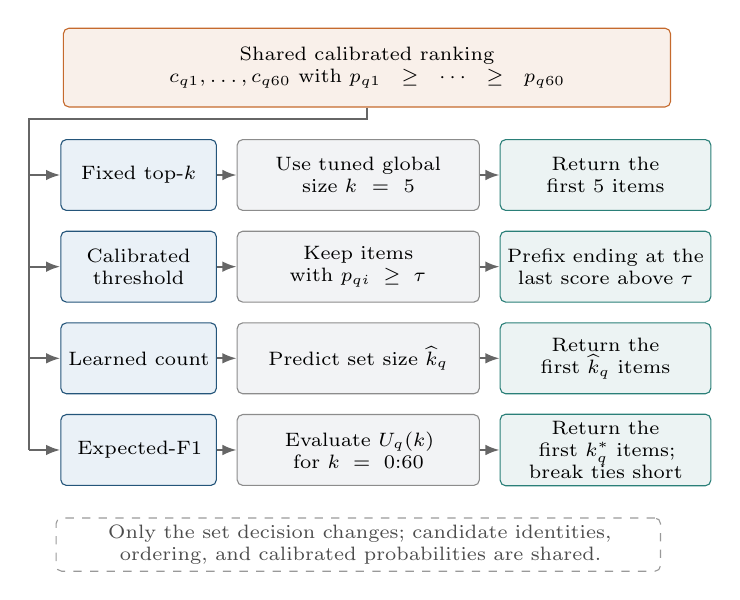
\begin{tikzpicture}[
  font=\scriptsize,
  policy/.style={draw=accentblue, rounded corners=2pt, fill=softblue,
    minimum height=9mm, text width=18mm, align=center, inner sep=2.5pt},
  rule/.style={draw=black!45, rounded corners=2pt, fill=softgray,
    minimum height=9mm, text width=29mm, align=center, inner sep=2.5pt},
  selected/.style={draw=accentteal, rounded corners=2pt, fill=accentteal!9,
    minimum height=9mm, text width=25mm, align=center, inner sep=2.5pt},
  shared/.style={draw=accentorange, rounded corners=2pt, fill=accentorange!10,
    minimum height=10mm, text width=75mm, align=center, inner sep=3pt},
  note/.style={draw=black!40, dashed, rounded corners=2pt,
    text width=75mm, align=center, inner sep=2.5pt, text=black!70},
  arrow/.style={-{Latex[length=1.8mm]}, thick, draw=black!60}
]

\node[shared] (ranking) {Shared calibrated ranking\\
$c_{q1},\ldots,c_{q60}$ with $p_{q1}\geq\cdots\geq p_{q60}$};

\node[policy, below=4mm of ranking, xshift=-29mm] (fixed) {Fixed top-$k$};
\node[rule, right=2.5mm of fixed] (fixedrule) {Use tuned global size $k=5$};
\node[selected, right=2.5mm of fixedrule] (fixedset) {Return the first 5 items};

\node[policy, below=2.5mm of fixed] (threshold) {Calibrated threshold};
\node[rule, right=2.5mm of threshold] (thresholdrule) {Keep items with $p_{qi}\geq\tau$};
\node[selected, right=2.5mm of thresholdrule] (thresholdset) {Prefix ending at the last score above $\tau$};

\node[policy, below=2.5mm of threshold] (count) {Learned count};
\node[rule, right=2.5mm of count] (countrule) {Predict set size $\widehat{k}_q$};
\node[selected, right=2.5mm of countrule] (countset) {Return the first $\widehat{k}_q$ items};

\node[policy, below=2.5mm of count] (expected) {Expected-F1};
\node[rule, right=2.5mm of expected] (expectedrule) {Evaluate $U_q(k)$ for $k=0{:}60$};
\node[selected, right=2.5mm of expectedrule] (expectedset) {Return the first $k_q^*$ items; break ties short};

\draw[arrow] (fixed) -- (fixedrule);
\draw[arrow] (fixedrule) -- (fixedset);
\draw[arrow] (threshold) -- (thresholdrule);
\draw[arrow] (thresholdrule) -- (thresholdset);
\draw[arrow] (count) -- (countrule);
\draw[arrow] (countrule) -- (countset);
\draw[arrow] (expected) -- (expectedrule);
\draw[arrow] (expectedrule) -- (expectedset);

\node[note, below=4mm of expectedrule, xshift=0mm] (scope)
{Only the set decision changes; candidate identities, ordering, and calibrated probabilities are shared.};

\coordinate (spinetop) at ([xshift=-4mm]fixed.west);
\coordinate (spinebottom) at ([xshift=-4mm]expected.west);
\draw[thick, draw=black!60] (ranking.south) -- ++(0,-1.5mm) -| (spinetop);
\draw[thick, draw=black!60] (spinetop) -- (spinebottom);
\draw[arrow] (spinetop) -- (fixed.west);
\draw[arrow] (spinetop |- threshold.west) -- (threshold.west);
\draw[arrow] (spinetop |- count.west) -- (count.west);
\draw[arrow] (spinebottom) -- (expected.west);
\end{tikzpicture}
}
    \caption{Decision policies applied to the same calibrated ranking. Fixed top-5 uses one global size; thresholding uses an absolute cutoff; learned count predicts the size; expected-F1 evaluates every prefix and returns the shortest utility-maximizing one. The displayed values illustrate the procedure; they are not measurements.}
    \label{fig:policy-decoding}
\end{figure}

\paragraph{Fixed top-$k$.}
We tune $k\in\{1,2,3,5,10,20,40,60\}$ and select the top $k$ candidates. The resulting control is top-5.

\paragraph{Calibrated threshold.}
For threshold $\tau$, the selector returns every item with $p_{qi}\geq\tau$, subject to the common packet limit. The threshold is selected from $\{0.1,\ldots,0.9\}$.

\paragraph{Learned count.}
A count model predicts the number of evidence items, after which the corresponding probability-ranked prefix is returned.

\paragraph{Expected-F1 decoding.}
Candidates are sorted by calibrated probability. For each prefix length $k$, a dynamic program computes the exact expected F1 under independent Bernoulli membership variables. The selected size is
\begin{equation}
k_q^*=\arg\max_{0\leq k\leq 60}
\mathbb{E}\!\left[F_1(S_{q,k},Y_q)\mid p_{q1:60}\right].
\label{eq:expected-f1}
\end{equation}
For prefix $S_{q,k}$, the utility can be written
\begin{equation}
U_q(k)=\mathbb{E}\!\left[
\frac{2T_{q,k}}{k+T_{q,k}+R_{q,k}}
\;\middle|\;p_{q1:60}\right],
\label{eq:expected-f1-utility}
\end{equation}
where $T_{q,k}$ is the number of relevant items inside the prefix and $R_{q,k}$ is the number outside it. Two Poisson-binomial recurrences compute their distributions and the expectation exactly. Ties retain the shorter prefix. This rule uses the full membership distribution rather than a single cutoff or a separately predicted count.

We also test two extensions. The first subtracts $\lambda k$ from expected utility. The second additionally subtracts $\gamma R(S_{q,k})$, where $R$ counts same-source redundancy. Size penalties span 0 to 0.10 and redundancy penalties span 0 to 0.005. These terms are retained as ablations because the fitted optima reveal whether extra decoder structure contributes beyond calibration.

\subsection{Decision Scope and Assumptions}

The comparison changes only the set decision. Candidate identities, ranks, feature values, scorer outputs, and validation claims are shared across policies. Expected-F1 assumes conditionally independent Bernoulli memberships and is restricted to prefixes of the frozen ranking; it neither reorders candidates nor retrieves a missing item. The released complete-gold mapping is treated as the evaluation target, although Sec.~\ref{sec:limitations} discusses possible annotation incompleteness. These boundaries distinguish a decoder error from a retrieval error and prevent an adaptive policy from receiving a more favorable candidate universe.

\subsection{Shared Verifier}

Evidence policies can improve set overlap while harming the downstream verdict. To isolate that possibility, one verifier architecture and training procedure is shared across policies. Only the selected evidence changes. We compare verdict macro-F1 on the same 1,490 claims and use a declared non-inferiority margin of $-0.01$ for expected-F1 relative to fixed top-5.

\section{Experimental Design}
\label{sec:setup}

\subsection{Frozen Protocols and Claim Boundary}

The diagnostic configuration was frozen on 4 November 2026 prior to its outcome bearing run. It stores data and model revisions, five claim-group partition seeds, retrieval depths, scorer families, calibration candidates, selector grids, evaluation metrics, bootstrap settings and stopping rules. The bounded retrieval repair, completeness-aware switch and stronger verifier were frozen on 9 November 2026 prior to checking their respective results. Prior to fitting the affected models, the numeric threshold grid and verifier architecture was captured. Any changes to the experiment or runs that fail are stored in an append-only experiment ledger.

External implementation was committed prior to development preparation and 5-seed train-only manifest was committed on 11th November 2026. That manifest includes hashes for code, configuration, archive, pre-join ranking, candidate, gold-map, and audit, and fails if input is a mix of train-development. The development matrix was then carried out 152 times on 12 November 2026.

The MOCHEG validation split released earlier in the project has been used and is not new validation evidence. The execution path has no formal-test annotations and they are sealed. There is no automatic approval of a formal-test-run based on the validation outcome.

\subsection{Independent External Protocol}

For seeds 13, 37, 73, 101 and 137, the claim sizes for AVerImaTeC training are deterministically partitioned as 55\% fit, 15\% calibration, 15\% model selection and 15\% internal holdout. The locked development run is run on the same candidates and membership scores for the train-selected fixed top-$k$, calibrated thresholding, calibrated expected-F1, uncalibrated expected-F1 and the completeness-aware switch. All development results do not affect the retrieval, fitting, calibration, packet width and policy parameters.

The four comparisons of claim are a multiplicity family: threshold minus fixed, expected-F1 minus threshold, calibrated minus uncalibrated expected-F1 and switch minus threshold. They both utilize 10,000 bootstrap draws, Bonferroni simultaneous intervals and Holm adjusted two-sided values. For an effect to be considered superior, the Threshold value must be $\geq +0.010$ and have a positive Adjusted lower bound. Expected-F1 must return at least 15\% fewer items and be at least $-0.010$ non-inferior. Switch superiority also demands that each of the seed effects is positive and that there is no increase in the mean set size. The margin for verifier preservation is also $-0.010$.

Gemma-3-27B (bfloat16) is used by the organizer's semantic evaluator. The 54.86~GB of weight files will not fit in the single GPU RTX~4090 with 24.56~GiB, and the organizer launcher requires two GPUs. In view of this, we present actual normalized-source diagnostics and class-wise verifier results, rather than a `replacement score' as official. The execution of the blind test is not in the authorized execution boundary.

\subsection{Baselines, Outcomes, and Selection Budgets}

Matched policies include fixed top-5, calibrated thresholding, learned count, calibrated expected-F1, uncalibrated expected-F1 and the packet-completeness-aware switch. The main result is that of claim-macro complete-gold evidence F1. Secondary outcomes are precision, recall, Jaccard similarity, exact-set match, selected count, calibration metrics, reachability and verdict macro-F1.

Only training roles will be used to select scorer and calibration. The repair will look at three weights per retrieval branch that have been declared. Thresholding searches $\{0.1,\ldots,0.9\}$ and the completeness cutoff searches five values declared. Weighted-fusion advancement gate passes so no other retrieval branch is opened. Once locked validation is seen, these budgets will not support any expansion based on outcomes.

The claim-level differences are first averaged over the five deterministic partitions in each of the comparisons. Then, a claim-aligned bootstrap resamples the 1,490 claims 10,000 times. Selector-superiority gate: All the following against calibrated thresholding: Evidence F1 $\geq +0.010$, Paired 95\% interval $> 0$, No increase in mean selected-set size, and No negative in any 5 partitions. The verifier's non-inferiority margin is $-0.010$. Both the lower bound for the whole interval aligned with the seed, and the lower bound for each of the seeds clearing the margin are reported.

\subsection{Robustness and Diagnostic Analyses}

The original diagnostic packet is also checked for widths 10 and 20, for text-only evidence and image-only evidence, for removing 25\% and 50\% of reachable gold deterministically, for promoting 5 distractors, for duplication of the top 3 distractors, and for 0.5 and 2.0 probability temperatures. Under these perturbations, fitted selectors remain the same. The conditions are tests of reachability, modality, contamination of ranking, duplication, and probability scale; they are not estimates of production shift.

After the primary comparison, there are validation claims for no, partial, and complete released-gold reachability. This is a post hoc and descriptive stratification. It encourages the pre-specified completeness-aware switch but doesn't make the previous subgroup finding a confirmatory statement.

\subsection{Implementation, Hardware, and Audit}

Each run is stored with the following pieces of information: candidate-level scores, calibrated probabilities, selected identifiers, claim level metrics, fitted parameters, environment metadata (Table~\ref{tab:environment}), formal-test access flags. Independent audits recompute population counts, set metrics, paired effects, and gate conditions from saved records. The label-blind ranking is performed prior to the gold joining. If the run fails, the partial output of the four runs is saved with the repair reason, instead of being overwritten.

\begin{table}[t]
\centering
\caption{Recorded environment for the bounded repair and stronger-verifier runs. Energy was not instrumented, so no physical-energy claim is made.}
\label{tab:environment}
\small
\setlength{\tabcolsep}{3.5pt}
\begin{tabular}{p{0.30\columnwidth}p{0.62\columnwidth}}
\toprule
Item & Recorded setting \\
\midrule
Operating system & Windows 11 (build 26300), 64-bit \\
CPU and memory & Intel Core i9-14900KF; 32 logical CPUs; 63.8 GiB RAM \\
GPU & NVIDIA RTX 4090; 24,564 MiB; driver 610.88 \\
Runtime & Python 3.13.14; NumPy 2.5.4 \\
Neural stack & PyTorch 2.14.1+cu130; Transformers 4.57.6 \\
Verifier & Full-batch Adam, 300 epochs, 64 hidden units, five seeds \\
Uncertainty & 10,000 claim-aligned bootstrap resamples \\
\bottomrule
\end{tabular}
\end{table}

On this machine, the weighted retrieval run time is 9.5 seconds, the candidate construction time is 8.4 seconds, the base selector evaluation time is 158.8 seconds, and the completeness switching time is 334.8 seconds, and the stronger verifier time is 246.9 seconds. These are not cross-system efficiency results, but wall-clock records for reproducing. The faithful organizer-store preparation takes 50.5 minutes for 793 training claims and 21.2 minutes for 152 development claims, while the locked 5-seed comparison takes 19 seconds after preparation. These times involve text encoding, reranking by a cross-encoder, and even scoring the actual images using SigLIP2. One development image of 144 million pixels (MP) results in a PIL safety warning, but is processed without exclusion, OOM or fallback.

\section{Results}
\label{sec:results}

\begin{figure*}[t]
    \centering
    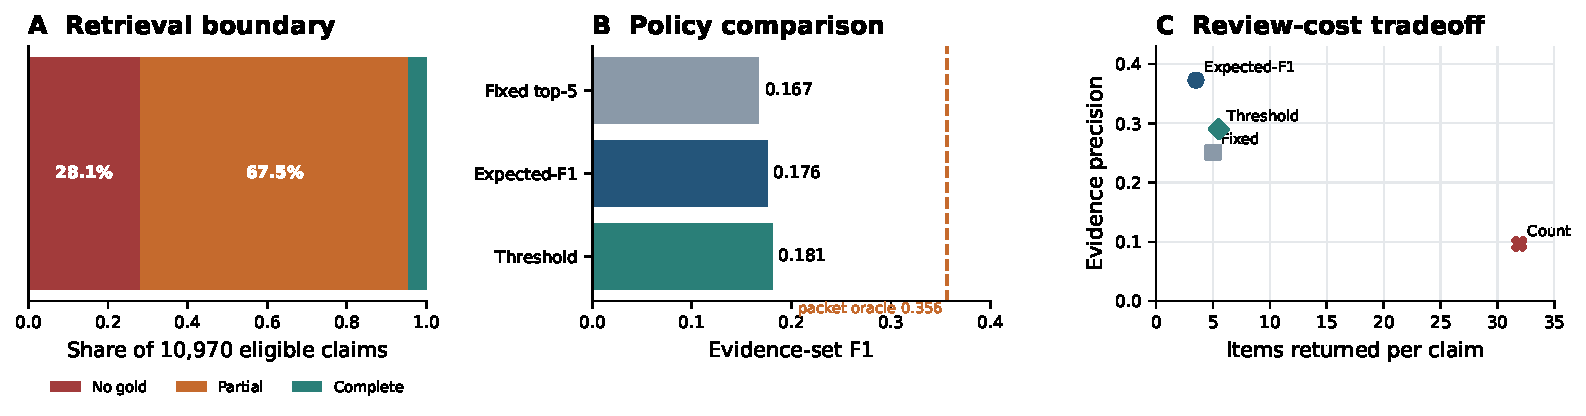
\includegraphics[width=\textwidth]{study_summary.pdf}
    \caption{Study at a glance. (A) Reachability over all 10,970 eligible claims; partial means at least one, but not all, released-gold items are present. (B) Locked-validation evidence F1 of the main policies, where the packet oracle is represented by the dashed boundary. (C) Precision and review-set-size tradeoff.}
    \label{fig:study-summary}
\end{figure*}

\subsection{Retrieval Defines a Low Ceiling}

At the actual operating depths of the selector, complete-gold recall for text is 0.3193 at 40 candidates and for images is 0.2663 at 20 candidates (Table~\ref{tab:operating-retrieval}). The combined packet has an oracle evidence F1 of 0.3560. Among the 10,970 eligible claims, only 4.39\% have all released gold items in the packet, while 3,086 have no reachable gold item. Most claims thus cannot be exactly recovered before set decoding starts.

\begin{table}[t]
\centering
\caption{Retrieval at the packet depths received by every selector.}
\label{tab:operating-retrieval}
\begin{tabular}{lrr}
\toprule
Modality & Retained depth & Complete-gold recall \\
\midrule
Text & 40 & 0.3193 \\
Image & 20 & 0.2663 \\
\bottomrule
\end{tabular}
\end{table}


The expanded retrieval audit also provides a better understanding of what parts are beneficial. Dense-BM25 RRF has a text Recall@50 of 0.3224. When reranking with a cross-encoder, it improves to 0.3338 while early Recall@5 decreases from 0.1772 to 0.1335. For images, SigLIP2-filename RRF achieves Recall@50 of 0.3149, whereas SigLIP2 gets 0.2183 and filename retrieval gets 0.2227. The text reranker sacrifices early ordering for greater recall; image fusion enhances retrieval.

\begin{table*}[t]
\centering
\caption{Complete-gold retrieval quality before packet truncation. Recall includes unretrieved released-gold items in the denominator; MAP and nDCG use the depth-100 ranked lists.}
\label{tab:retrieval-matrix}
\small
\setlength{\tabcolsep}{5pt}
\begin{tabular}{llrrrrrr}
\toprule
Modality & Retriever & R@5 & R@10 & R@20 & R@50 & MAP@100 & nDCG@100 \\
\midrule
Text & Dense sentence & 0.1767 & 0.2141 & 0.2523 & 0.3028 & 0.1728 & 0.2972 \\
Text & BM25 sentence & 0.1452 & 0.1744 & 0.2048 & 0.2478 & 0.1349 & 0.2409 \\
Text & Dense + BM25 RRF & 0.1772 & 0.2194 & 0.2659 & 0.3224 & 0.1744 & 0.3031 \\
Text & RRF + cross-encoder & 0.1335 & 0.1915 & 0.2574 & 0.3338 & 0.1282 & 0.2587 \\
Image & SigLIP2 & 0.1145 & 0.1436 & 0.1782 & 0.2183 & 0.0916 & 0.1312 \\
Image & Filename dense & 0.1408 & 0.1653 & 0.1889 & 0.2227 & 0.1154 & 0.1490 \\
Image & SigLIP2 + filename RRF & 0.1904 & 0.2292 & 0.2663 & 0.3149 & 0.1414 & 0.1938 \\
\bottomrule
\end{tabular}
\end{table*}


As shown in Table~\ref{tab:retrieval-matrix}, the two branches, text and image, fail differently. Text RRF improves both MAP and nDCG over the first-stage models, while the cross-encoder gains deeper Recall@50 at the cost of early precision-sensitive ordering. Image fusion enhances all the reported cutoffs and both ranking metrics, yet its Recall@50 is still below the text branch. This means that a larger packet would contain some evidence that might be missing, but would also reveal a more challenging distractor distribution for the selector.

\begin{table*}[t]
\centering
\caption{Locked-validation performance by packet reachability. The packet oracle selects every reachable released-gold item. Selector values average claim-level F1 across five deterministic training-role partitions.}
\label{tab:reachability-strata}
\begin{tabular}{lrrrrr}
\toprule
Reachability stratum & Claims (share) & Packet oracle & Fixed top-5 & Threshold & Expected-F1 \\
\midrule
No gold reachable & 211 (14.2\%) & 0.000 & 0.000 & 0.000 & 0.000 \\
Partially reachable & 1,200 (80.5\%) & 0.466 & 0.184 & 0.196 & 0.184 \\
Complete gold reachable & 79 (5.3\%) & 1.000 & 0.359 & 0.424 & 0.524 \\
\bottomrule
\end{tabular}
\end{table*}


Table~\ref{tab:reachability-strata} shows how adaptive selection comes in handy in the post hoc validation stratification. For the 79 claims where the entire released-gold set can be obtained, expected-F1 is 0.5240 F1, compared with 0.3593 for fixed top-5 and 0.4237 for thresholding. On the 1,200 partially reachable claims, expected-F1 is 0.1839 and does not improve on fixed top-5 at 0.1841; thresholding is best at 0.1965. The 211 claims where the gold is not reachable have a score of zero for all methods. The aggregate expected-F1 gain is thus localized in the small complete-reachability stratum, while thresholding is more effective for incomplete packets.

\subsection{Prior-Aware Maps Repair Calibration}

Table~\ref{tab:calibration} makes a comparison between maps on locked validation, averaged over modalities and deterministic partitions. Brier scores for identity and temperature are 0.0847 and 0.0832, respectively. They differ by a small amount, consistent with a prior error for which a slope-only temperature is not a cure. Isotonic, Platt and prior-shift calibration further lower the Brier score to around 0.033, and improve the NLL and ECE. When compared to identity calibration, isotonic calibration decreases Brier error by approximately 61\% and ECE from 0.1314 to 0.0063. All five partitions have positive Brier skill relative to the prevalence-only reference, with partition-level skill of roughly 14\%.

\begin{table}[t]
\centering
\caption{Validation calibration averaged across modalities and deterministic partitions.}
\label{tab:calibration}
\begin{tabular}{lrrr}
\toprule
Map & Brier $\downarrow$ & NLL $\downarrow$ & ECE $\downarrow$ \\
\midrule
Isotonic & 0.0330 & 0.1301 & 0.0063 \\
Platt & 0.0331 & 0.1302 & 0.0067 \\
Prior Shift & 0.0331 & 0.1305 & 0.0076 \\
Beta & 0.0359 & 0.3377 & 0.0198 \\
Temperature & 0.0832 & 0.2830 & 0.1220 \\
Identity & 0.0847 & 0.2837 & 0.1314 \\
\bottomrule
\end{tabular}
\end{table}


\begin{figure}[t]
    \centering
    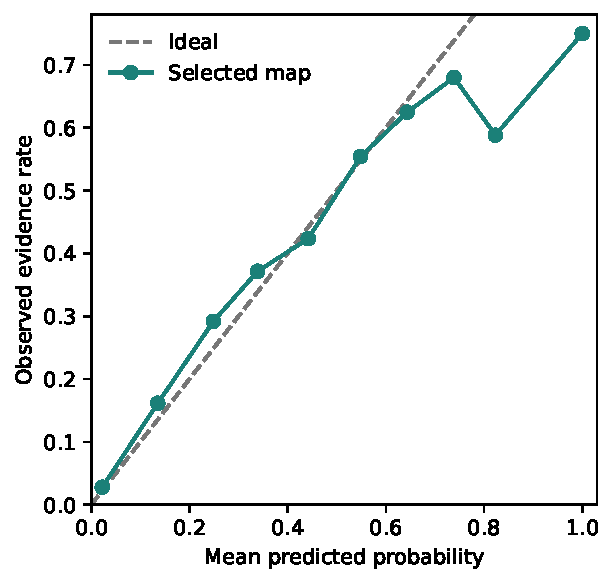
\includegraphics[width=\columnwidth]{calibration_reliability.pdf}
    \caption{Reliability on locked validation. Temperature scaling is still overconfident as it is unable to correct the class-prior shift. Prior-shift, Platt and isotonic maps closely approximate the observed membership rate.}
    \label{fig:calibration}
\end{figure}

Also, after enforcing absolute calibration, scorer choice changes. Partitions 13 and 37 use modality-specific balanced models, while 73 uses an unweighted cross-encoder model, and 101 and 137 use unweighted modality-specific models. For text maps, there is variation between isotonic, Platt and beta maps, while for image scoring, the map is isotonic in all five partitions. This variation may be helpful in considering scorer family, loss weighting, and calibration as a single selection problem.

\subsection{Adaptive Selection Helps, but Thresholding Wins}

The important locked-validation results are shown in Table~\ref{tab:selector-means}. Fixed top-5 reaches 0.1673 evidence F1. Expected-F1 reaches 0.1759 while selecting just 3.50 items per claim. Its precision rises from 0.2511 to 0.3725, while recall falls from 0.1753 to 0.1483. Expected-F1 trades recall for increased precision and a smaller review set.

The highest F1 is achieved by calibrated thresholding, which selects 5.51 items and has an F1 of 0.1807. Learned count prediction selects 31.90 items and gets 0.1100 F1. Without a well-matched set objective, it is not competitive to predict the size.

\begin{table*}[t]
\centering
\caption{Locked-validation evidence-set results over 1,490 claims. Values are means across five deterministic training-role partitions.}
\label{tab:selector-means}
\begin{tabular}{lrrrrr}
\toprule
Method & Precision & Recall & F1 & Exact match & Selected \\
\midrule
Fixed top-5 & 0.2511 & 0.1753 & 0.1673 & 0.0000 & 5.00 \\
Calibrated threshold & 0.2898 & 0.1798 & 0.1807 & 0.0036 & 5.51 \\
Learned count & 0.0965 & 0.2791 & 0.1100 & 0.0001 & 31.90 \\
Expected-F1 & 0.3725 & 0.1483 & 0.1759 & 0.0093 & 3.50 \\
Size-penalized expected-F1 & 0.3725 & 0.1483 & 0.1759 & 0.0093 & 3.50 \\
Size + redundancy expected-F1 & 0.3725 & 0.1483 & 0.1759 & 0.0093 & 3.50 \\
\bottomrule
\end{tabular}
\end{table*}


\begin{table*}[t]
\centering
\caption{Partition-level locked-validation evidence selection. Every row contains the same 1,490 validation claims; partitions change only the training, calibration, and model-selection roles.}
\label{tab:partition-selector-results}
\small
\setlength{\tabcolsep}{5pt}
\begin{tabular}{rrrrrrrr}
\toprule
Partition & Fixed F1 & Threshold F1 & Expected-F1 & Difference & Precision & Recall & Selected \\
\midrule
13 & 0.1677 & 0.1814 & 0.1766 & +0.0089 & 0.3727 & 0.1484 & 3.56 \\
37 & 0.1682 & 0.1811 & 0.1758 & +0.0076 & 0.3774 & 0.1480 & 3.48 \\
73 & 0.1660 & 0.1791 & 0.1761 & +0.0101 & 0.3746 & 0.1476 & 3.43 \\
101 & 0.1674 & 0.1800 & 0.1756 & +0.0082 & 0.3666 & 0.1493 & 3.59 \\
137 & 0.1674 & 0.1818 & 0.1751 & +0.0077 & 0.3714 & 0.1480 & 3.45 \\
\bottomrule
\end{tabular}
\end{table*}


The expected-F1 effect is consistent across the partition-level results in Table~\ref{tab:partition-selector-results}. It has a stable precision-recall profile, a gain of $+0.0076$ to $+0.0101$ over fixed top-5 and a size range of 3.43 to 3.59. The method returns approximately 30\% fewer items on average and improves F1 by approximately 5.1\% relative to fixed top-5. There is no change in the baseline ordering, as thresholding always wins.

The claim-aligned effects in Table~\ref{tab:selector-effects-detail} and Fig.~\ref{fig:selector-effects} confirm these differences. Expected-F1 improves on fixed top-5 by $0.00851$ with a 95\% interval of $[0.00302,0.01400]$ and Holm-adjusted $p=0.0078$. Thresholding improves by $0.01334$ $[0.00931,0.01744]$. Its direct advantage over expected-F1 is $0.00483$ $[0.00003,0.00957]$.

\begin{table}[t]
\centering
\caption{Claim-aligned evidence-F1 effects against fixed top-5.}
\label{tab:selector-effects-detail}
\resizebox{\columnwidth}{!}{%
\begin{tabular}{lrrr}
\toprule
Method & Mean & 95\% interval & Holm $p$ \\
\midrule
Calibrated threshold & +0.0133 & [+0.0093, +0.0174] & 0.0010 \\
Learned count & -0.0574 & [-0.0641, -0.0507] & 0.0010 \\
Expected-F1 & +0.0085 & [+0.0030, +0.0140] & 0.0078 \\
Size-penalized expected-F1 & +0.0085 & [+0.0029, +0.0141] & 0.0078 \\
Size + redundancy expected-F1 & +0.0085 & [+0.0029, +0.0141] & 0.0078 \\
\bottomrule
\end{tabular}%
}
\end{table}


\begin{figure}[t]
    \centering
    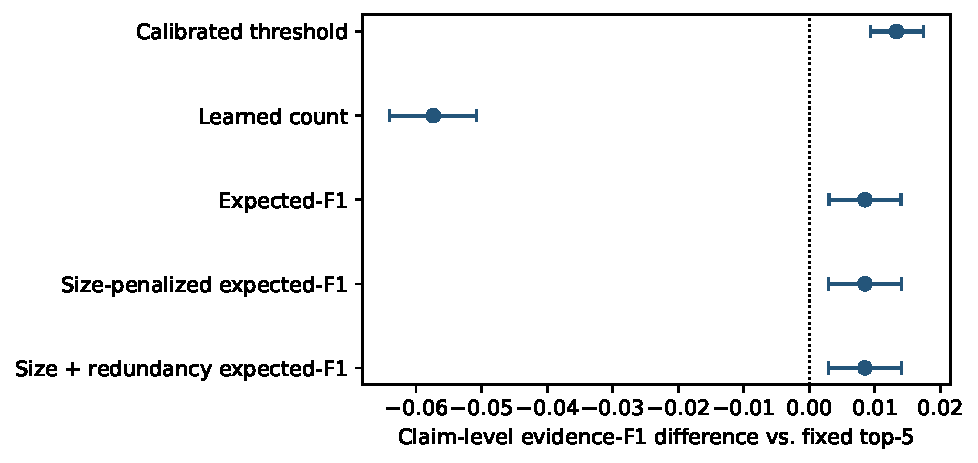
\includegraphics[width=\columnwidth]{corrected_selector_effects.pdf}
    \caption{Claim-aligned evidence-F1 effects with respect to fixed top-5. Points are mean differences and bars are 95\% intervals.}
    \label{fig:selector-effects}
\end{figure}

Both penalty extensions are a perfect match with plain expected-F1. In each partition, the selected size penalty is zero and the selected redundancy penalty is zero. The extra terms introduced complexity without altering the answer on this packet, as can be seen from their claim-level outputs. The quantifiable improvement is through calibrated probabilities.

There is not sufficient evidence to support the superiority condition. Despite the fact that expected-F1 is positive in all partitions and that the corrected interval does not contain zero, it still has a mean gain of 0.00851, which is less than the stated target of 0.015. This experiment therefore provides a small positive development effect, but not enough to surpass the superiority threshold.

\begin{figure*}[!t]
    \centering
    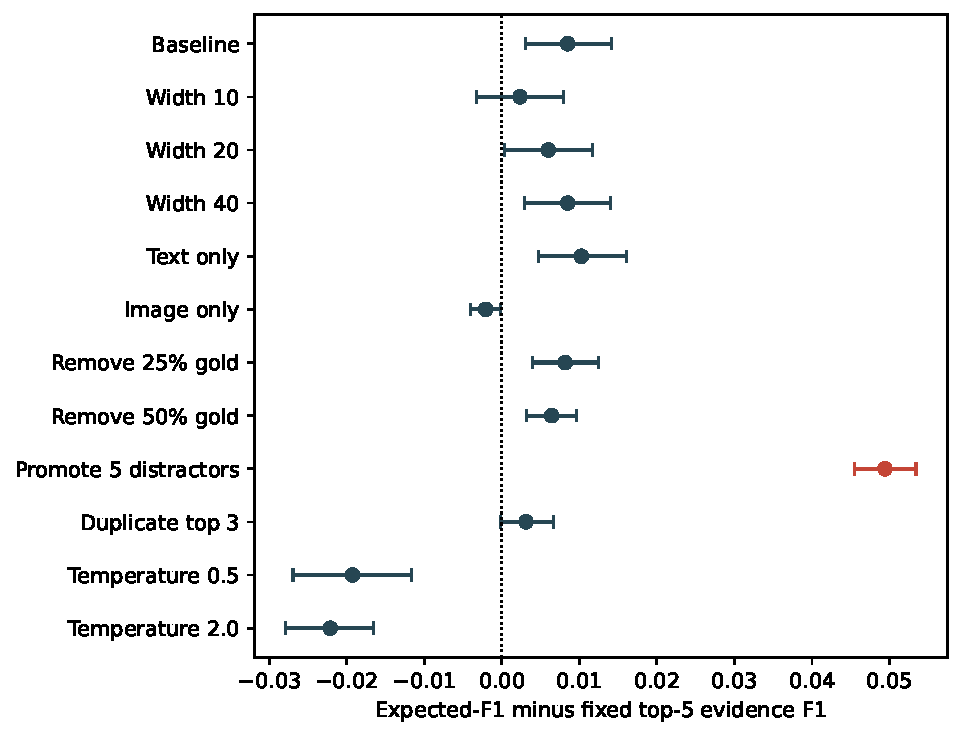
\includegraphics[width=\textwidth]{robustness_effects.pdf}
    \caption{Expected-F1 minus fixed top-5 under controlled perturbations. Probability-temperature changes reverse the baseline gain without changing the candidate ranking.}
    \label{fig:robustness}
\end{figure*}

\subsection{The Verifier Safeguard Remains Unresolved}

We find that the mean difference between expected-F1 and fixed top-5 is $+0.00099$ with a 95\% interval of $[-0.01053,+0.01279]$ under the shared verifier. The lower limit is just below the stated non-inferiority margin of $-0.01$. The point estimate is not far from zero, but the interval does not establish that verdict quality was preserved. Threshold-selected evidence has the highest verifier macro-F1 in every partition (Table~\ref{tab:verifier-effects}).

\begin{table}[t]
\centering
\caption{Shared-verifier macro-F1 by deterministic partition.}
\label{tab:verifier-effects}
\begin{tabular}{lrrrr}
\toprule
Partition & Fixed & Threshold & Expected-F1 & Difference \\
\midrule
13 & 0.3499 & 0.3634 & 0.3472 & -0.0027 \\
37 & 0.3478 & 0.3602 & 0.3525 & +0.0047 \\
73 & 0.3494 & 0.3695 & 0.3488 & -0.0006 \\
101 & 0.3578 & 0.3674 & 0.3579 & +0.0001 \\
137 & 0.3564 & 0.3699 & 0.3598 & +0.0034 \\
\bottomrule
\end{tabular}
\end{table}


\begin{figure}[t]
    \centering
    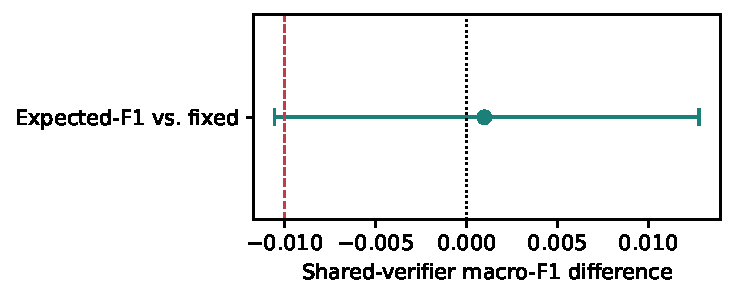
\includegraphics[width=\columnwidth]{corrected_verifier_effect.pdf}
    \caption{Shared-verifier effect of expected-F1 evidence relative to fixed top-5. The $-0.01$ non-inferiority margin is indicated by a dashed line.}
    \label{fig:verifier}
\end{figure}

\subsection{Robustness Exposes Calibration Sensitivity}

There is a positive effect of expected-F1 under width 20 and 40, text-only evidence, and deterministic gold removal. It falls slightly behind fixed top-5 on image-only packets. The impact of promoting five distractors is much bigger because fixed top-5 collapses when all five top positions are filled with distractors; this should not be interpreted as the normal operating impact.

The results are most sensitive to probability perturbations. Sharpening the probabilities with a temperature of 0.5 makes the effect $-0.0193$, and flattening with a temperature of 2.0 makes the effect $-0.0221$. The intervals do not include zero. Expected-F1 is therefore sensitive to probability scale, which does not change candidate order.

Prior-aware maps correct the dominant calibration error and retrieval becomes a hard constraint on the performance that can be achieved. Calibrated expected-F1 offers a slight precision-oriented gain compared to fixed top-5, which is mostly based on claims with full reachable gold. Calibrated thresholding is stronger overall. The advantage depends on probability quality and still does not meet the verifier safeguard.

\clearpage

\section{Independent External Evaluation}
\label{sec:external-results}

AVerImaTeC changes the evidence unit, candidate store, output cap, and verdict label space. The prespecified comparisons use one locked development evaluation of five train-only seeds (Fig.~\ref{fig:external-summary}). The subsequent calibration and failure analyses reuse frozen models and outputs. The evidence diagnostics use exact normalized URLs and released image basenames. Full semantic scoring is outside the reported comparison.

\begin{figure*}[t]
    \centering
    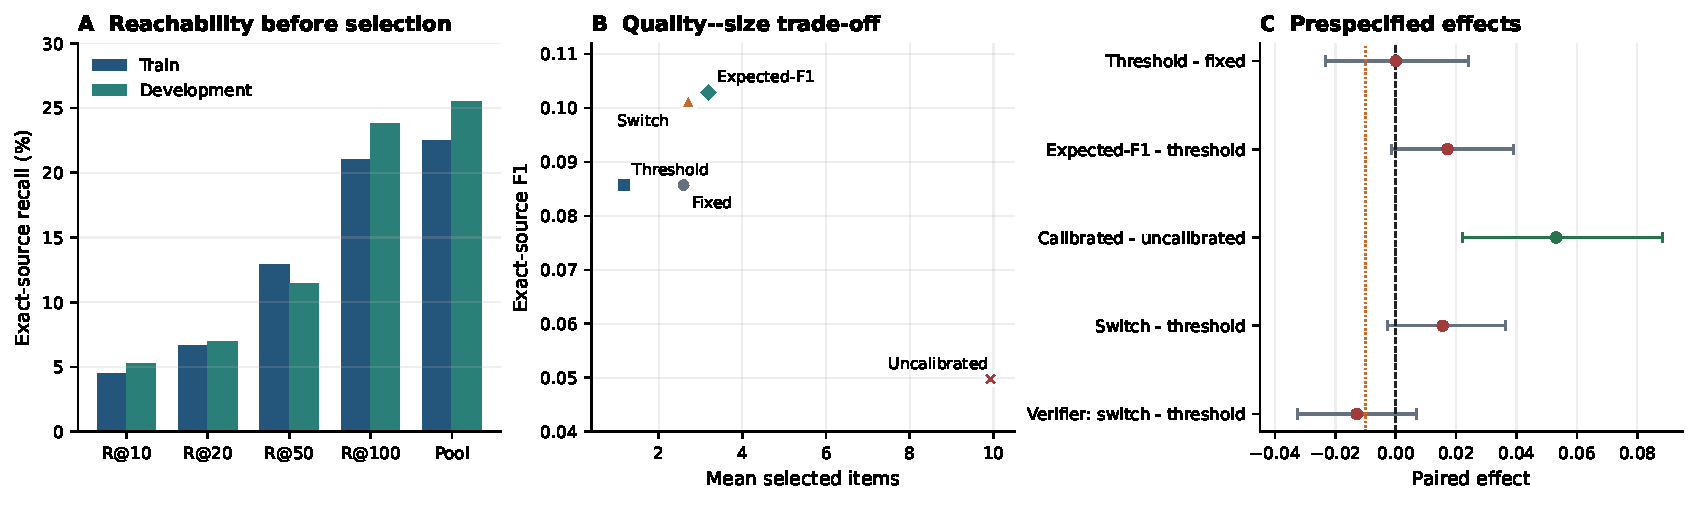
\includegraphics[width=\textwidth]{external_confirmation_summary.pdf}
    \caption{Independent AVerImaTeC development results. (a) Exact-source reachability before selection. (b) Calibrated expected-F1 has the highest diagnostic F1. Uncalibrated expected-F1 nearly reaches the ten-item cap. (c) Only the calibration effect has a positive multiplicity-adjusted interval. The verifier uses an unadjusted seed-aligned 95\% interval}
    \label{fig:external-summary}
\end{figure*}

\subsection{The Organizer Store Does Not Remove the Retrieval Ceiling}

We discovered 529,580 text and 81,817 image candidates for 793 training claims, and 101,289 text and 49,617 image candidates for 152 development claims. Each development claim has store candidates. Table~\ref{tab:external-reachability} shows how often the ranked pool contains the annotated identities.

\begin{table}[t]
\centering
\caption{Exact-source reachability before selection. Training means use 792 claims with nonempty web-source gold; development uses all 152 claims.}
\label{tab:external-reachability}
\small
\setlength{\tabcolsep}{3pt}
\begin{tabular}{@{}lrrrr@{}}
\toprule
Split & \shortstack{Pool\\recall} & Complete & Zero & \shortstack{Recall\\@100} \\
\midrule
Training & 0.2247 & 0.0922 & 0.6136 & 0.2105 \\
Development & 0.2548 & 0.1250 & 0.5987 & 0.2378 \\
\bottomrule
\end{tabular}
\end{table}

Development Recall@10, @20, and @50 is 0.0526, 0.0696, and 0.1143. The ranked pool of 100 text and 20 image candidates yields 25.48\% claim-macro recall. It contains every exact target for 19 claims and contains none for 91. This is the recall ceiling before the scorer forms a smaller packet for selection.

\subsection{Calibration on Frozen Development Candidates}

We replayed the frozen scorer and calibration map for each seed on the 18,240 ranked candidates. Table~\ref{tab:external-cal} reports candidate-weighted metrics computed per seed and averaged over seeds. The combined results pool candidate rows across modalities within each seed. Expected calibration error (ECE) uses ten equal-width probability bins, and negative log-likelihood (NLL) clips probabilities to $[10^{-12},1-10^{-12}]$. The development prevalence baseline predicts the observed positive fraction within each evaluation population and supplies a descriptive reference.

\begin{table*}[t]
\centering
\caption{Post hoc AVerImaTeC calibration on exact candidate membership. The baseline Brier score uses development prevalence. AP is average precision. Image AP is undefined because the pool contains zero exact-positive images.}
\label{tab:external-cal}
\small
\setlength{\tabcolsep}{4pt}
\begin{tabular}{llrrrrrrr}
\toprule
Candidates & Scores & Rows & Positive & Brier & Baseline Brier & NLL & ECE & AP \\
\midrule
Text & Raw & 15,200 & 86 & .18419 & .00563 & .56806 & .39639 & .06751 \\
 & Calibrated & & & .00546 & & .02948 & .00077 & .06751 \\
\addlinespace
Image & Raw & 3,040 & 0 & .00547 & 0 & .07467 & .07178 & -- \\
 & Calibrated & & & $1.44{\times}10^{-7}$ & & .00030 & .00030 & -- \\
\addlinespace
Combined & Raw & 18,240 & 86 & .15440 & .00469 & .48583 & .34229 & .06751 \\
 & Calibrated & & & .00455 & & .02461 & .00066 & .06751 \\
\bottomrule
\end{tabular}
\end{table*}

Calibration sharply reduces overconfidence and yields a combined Brier score about 3\% below the descriptive prevalence reference. AP is unchanged, consistent with an improvement in probability scale on this population. The image result reflects lower predicted probabilities on exact negatives. Positive-image probability quality remains unmeasured.

\subsection{Matched Evidence-Set Decisions}

Table~\ref{tab:external-selectors} averages within each claim over the five frozen seeds, then over claims. Calibrated expected-F1 has the highest point estimate (0.1029) at 3.20 unique identities per claim. Thresholding returns the smallest sets (1.17). Uncalibrated expected-F1 nearly fills the ten-item cap and reaches 0.0497 F1.

A modality audit found only text in the 3,800 frozen policy outputs, although the ranked pool included image candidates. The external selection comparison therefore measures policy behavior on text selections for multimodal claims. It leaves the value of selected visual evidence open.

\begin{table*}[t]
\centering
\caption{Exact-source results on locked AVerImaTeC development, averaged over five train-only seeds.}
\label{tab:external-selectors}
\small
\setlength{\tabcolsep}{7pt}
\begin{tabular}{lccccc}
\toprule
Policy & Precision & Recall & F1 & Exact set & Items \\
\midrule
Train-selected fixed top-$k$ & 0.0846 & 0.1116 & 0.0857 & 0.0053 & 2.59 \\
Calibrated threshold & \textbf{0.1308} & 0.0725 & 0.0857 & \textbf{0.0289} & \textbf{1.17} \\
Calibrated expected-F1 & 0.1198 & 0.1214 & \textbf{0.1029} & 0.0145 & 3.20 \\
Uncalibrated expected-F1 & 0.0306 & \textbf{0.1614} & 0.0497 & 0.0000 & 9.93 \\
Completeness-aware switch & 0.1208 & 0.1160 & 0.1013 & 0.0145 & 2.71 \\
\bottomrule
\end{tabular}
\end{table*}

Table~\ref{tab:external-decisions} reports 10,000 paired claim-bootstrap draws with 98.75\% per-comparison intervals for 95\% simultaneous coverage and Holm-adjusted $p$-values. Threshold superiority remains unestablished. Expected-F1 clears the $-0.010$ non-inferiority margin against thresholding and misses the compactness gate, returning about 174\% more identities. The calibration ablation clears its gate. The switch improves the point estimate in each seed, while its adjusted interval crosses zero.

\begin{table*}[t]
\centering
\caption{Prespecified external comparison family. CI denotes the simultaneous interval after Bonferroni correction.}
\label{tab:external-decisions}
\small
\setlength{\tabcolsep}{5pt}
\begin{tabular}{lrrrc}
\toprule
Comparison & Mean effect & Simultaneous CI & Holm $p$ & Gate \\
\midrule
Threshold $-$ fixed & $+0.00003$ & $[-0.02341,\,0.02404]$ & 0.9989 & \fail \\
Expected-F1 $-$ threshold & $+0.01714$ & $[-0.00148,\,0.03905]$ & 0.0714 & compactness \fail \\
Calibrated $-$ uncalibrated expected-F1 & $+0.05316$ & $[0.02207,\,0.08852]$ & 0.0008 & \pass \\
Switch $-$ threshold & $+0.01555$ & $[-0.00263,\,0.03621]$ & 0.0714 & \fail \\
\bottomrule
\end{tabular}
\end{table*}

\subsection{The Downstream Safeguard Fails Externally}

The mean verifier macro-F1 is 0.1573 (threshold evidence) and 0.1444 (switch evidence) (Table~\ref{tab:external-verifier}). The seed-aligned switch-minus-threshold effect is $-0.01293$ with 95\% interval $[-0.03242,0.00687]$ which does not exceed the reported $-0.010$. The switch therefore fails verifier non-inferiority, unlike the aggregate MOCHEG result.

\begin{table*}[t]
\centering
\caption{Five-seed mean four-class verifier results on locked development. CE/C denotes Conflicting Evidence/Cherrypicking.}
\label{tab:external-verifier}
\begin{tabular}{lrrrrrr}
\toprule
Evidence policy & Acc. & Macro-F1 & Sup. & Ref. & NEI & CE/C \\
\midrule
Threshold & 0.3158 & \textbf{0.1573} & 0.1150 & 0.4710 & 0.0432 & 0.0000 \\
Switch & 0.2842 & 0.1444 & 0.1000 & 0.4300 & 0.0474 & 0.0000 \\
\bottomrule
\end{tabular}
\end{table*}

The development split contains 141 Refuted, six Not Enough Evidence, four Supported, and one Conflicting claim. Both policies miss the Conflicting example in all five seeds. We report class-wise results and macro-F1 because accuracy alone gives little information about the rare verdicts.

\subsection{Where Exact Evidence Was Lost}

We traced 337 claim--target identities through the indexed store, usable candidate discovery, ranked pool, scorer packet, and saved selections. Each seed repeats the same store and pool, giving 1,685 target--seed instances. We counted each target once at its first failure stage (Fig.~\ref{fig:external-diagnostics}). Store presence means a normalized URL in the claim-indexed store entries or an exact image basename. A URL was usable if its record yielded a nonempty text segment. Basename absence cannot resolve visual equivalence.

Fourteen identities were absent by this definition, including all eight annotated image identities. A further 93 had a store URL but no usable candidate text, and 153 were discovered but ranked outside the retained pool. The store listed every exact identity for 145 of 152 claims, the usable candidates covered 79, and the pool covered 19. The scorer packet contained the complete set in 80 of 760 claim--seed instances (10.53\%). Under fixed selection, 52 target--seed instances fell outside that packet, 178 were omitted by the selector, and 155 were selected. These counts distinguish acquisition and ranking losses from selection opportunities.

\begin{figure*}[t]
\centering
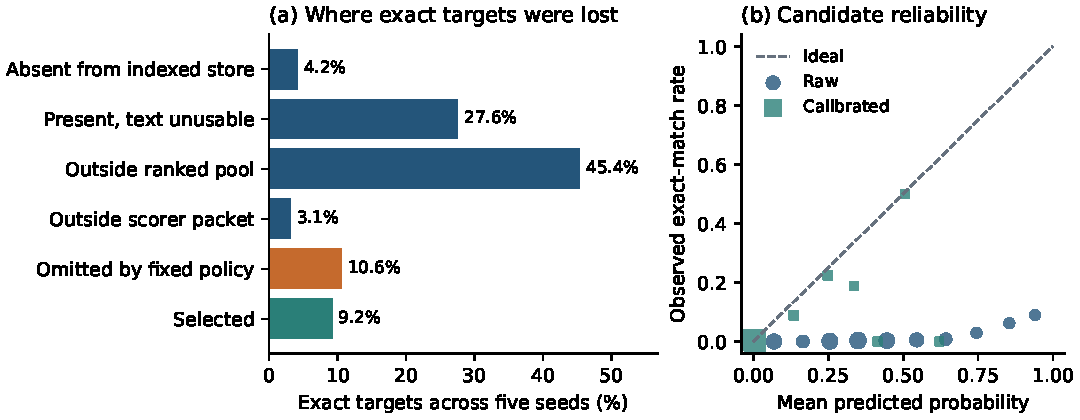
\includegraphics[width=0.93\textwidth]{one_shot_external_diagnostics.pdf}
\caption{Post hoc diagnostics on frozen AVerImaTeC development outputs. (a) Each exact target--seed instance is counted once under the fixed policy. (b) Pooled reliability across candidate rows and seeds. Point area reflects bin support, and the dashed line indicates ideal calibration}
\label{fig:external-diagnostics}
\end{figure*}

Among claim--seed instances with at least one selected exact target, the verifier made 59 errors in 103 instances under thresholding and 103 in 153 under the switch. These are claim-level associations under a shared verifier. Exact overlap can coexist with incomplete or unhelpful evidence.

\subsection{Cross-Benchmark Transfer}

Table~\ref{tab:cross-benchmark} aligns the research questions across development protocols. The metrics remain specific to each benchmark's evidence unit. Table~\ref{tab:external-disagreement} shows that the policies often return different sources even when every annotated identity is missing from the ranked pool.

\begin{table*}[t]
\centering
\caption{Development findings across benchmarks, using each benchmark's evidence units. MOCHEG and verifier intervals are paired 95\% intervals. External selector intervals use the four-comparison correction.}
\label{tab:cross-benchmark}
\small
\begin{tabular}{@{}>{\raggedright\arraybackslash}p{0.20\textwidth}*{2}{>{\raggedright\arraybackslash}p{0.365\textwidth}}@{}}
\toprule
Question & MOCHEG (1,490 claims) & AVerImaTeC (152 claims) \\
\midrule
Reachability & Text R@40 .3393 and image R@20 .3287. Complete 5.91\%, zero 13.89\%. & Pooled exact-source claim-macro recall .2548. Complete 12.50\%, zero 59.87\%. \\
Probability quality & Identity to isotonic mean Brier .0847 to .0330. Selected maps have positive Brier skill against prevalence in every partition. & Raw to frozen-map combined mean Brier .15440 to .00455, with .00469 for development prevalence. \\
Threshold vs.\ fixed & $+.01517$ $[.01114,.01923]$. & $+.00003$ $[-.02341,.02404]$. \\
Expected-F1 vs.\ threshold & $-.00484$ $[-.00938,-.00020]$ with 3.61 vs.\ 5.26 items. & $+.01714$ $[-.00148,.03905]$ with 3.20 vs.\ 1.17 identities. \\
Switch vs.\ threshold & $+.00138$ $[-.00191,.00462]$. Superiority gate fails. & $+.01555$ $[-.00263,.03621]$. Superiority gate fails. \\
Verifier preservation & $+.00434$ $[-.00277,.01130]$ macro-F1. Aggregate margin clears, seed safeguard fails. & $-.01293$ $[-.03242,.00687]$ macro-F1. Aggregate margin fails. \\
\bottomrule
\end{tabular}
\end{table*}

\begin{table}[t]
\centering
\caption{Policy disagreement by ranked-pool exact reachability. Each cell gives unequal source sets out of the indicated claim--seed denominator.}
\label{tab:external-disagreement}
\small
\setlength{\tabcolsep}{3pt}
\begin{tabular}{@{}lrrr@{}}
\toprule
Policy vs.\ threshold & Zero & Partial & Complete \\
\midrule
Fixed & 349/455 & 167/210 & 72/95 \\
Expected-F1 & 384/455 & 144/210 & 74/95 \\
Switch & 308/455 & 124/210 & 64/95 \\
\bottomrule
\end{tabular}
\end{table}

\subsection{Frozen Decision}

Under the frozen decision rule, the switch requires superiority and verifier preservation, expected-F1 requires non-inferiority and at least 15\% fewer identities than thresholding, and thresholding requires superiority over fixed selection. The rule defaulted to the train-selected fixed family. Its five local development exports meet the organizer's ten-item and 1,500-character limits. Formal test annotations remain sealed.

\section{Discussion}
\label{sec:discussion}

\subsection{Calibration Changes the Decision, Not the Ranking}

Expected-F1 requires probabilities with operational meaning: among items given
probability 0.30, roughly 30\% should be evidence members under comparable
conditions. Balanced logistic training improves rare-positive ranking but
changes the effective training prior. Temperature scaling changes logit slope,
whereas prior shift, Platt, beta, and isotonic mappings can also repair the
location or shape of the reliability curve. The uncalibrated expected-F1
ablation makes this distinction concrete: it selects nearly 25 items per claim
and loses more than five evidence-F1 points relative to calibrated
expected-F1, with no change to the candidate universe.

This is the one relationship that reproduces cleanly on AVerImaTeC. There,
uncalibrated expected-F1 nearly saturates the ten-item cap and loses 0.0532
exact-source F1 to its calibrated counterpart. The positive simultaneous
interval survives multiplicity correction despite different candidate units,
class balance, and independently fitted models. Calibration is therefore not
an explanation fitted only to the MOCHEG packet.

This also explains why fitted size and redundancy penalties are unnecessary in
the diagnostic experiment. Once the low membership prevalence is restored,
the unpenalized expected utility already favors a short prefix. Adaptive
selector studies should report probability quality, prevalence, and selected
set size alongside rank metrics; otherwise the decoder can appear to improve
or fail for the wrong reason.

\subsection{Why Thresholding Remains the Strong Baseline}

Expected-F1 combines all membership probabilities under a conditional-
independence approximation. A tuned threshold uses the same calibrated
probabilities with fewer structural assumptions. On the repaired packet,
thresholding is 0.00484 F1 stronger and recovers more evidence, while
expected-F1 returns 1.64 fewer items and has higher precision. The latter is a
valid review-cost operating point, but it is not the strongest selector by the
primary metric.

The external result narrows this conclusion. AVerImaTeC thresholding returns
the smallest set but is tied with the train-selected fixed family, whereas
expected-F1 reaches a higher point estimate by selecting 3.20 rather than 1.17
items. Expected-F1 clears the non-inferiority margin but fails the required
size reduction. Thresholding remains a necessary comparator, not a universally
superior policy, and compactness does not transfer automatically.

The completeness-aware switch tests whether these policies can be combined
without simply choosing the better one on validation. Its point estimate is
higher than thresholding and its mean set is smaller, but the improvement is
too small and unstable to support superiority. This negative result is useful:
packet completeness is a plausible routing variable, yet the present ten-
feature logistic estimate is not accurate enough to produce a reliable
method-level gain. A future model should first improve completeness prediction
under a frozen protocol, rather than add another decoder penalty.

\subsection{Retrieval Is Still the Dominant Constraint}

Weighted fusion reduces zero-reachable claims and raises the packet oracle, but
the all-eligible ceiling remains only 0.3637 F1 and complete-gold coverage
remains below 5\%. The absolute gain is far smaller than the declared
engineering target. Most selector errors therefore cannot be repaired by a
different prefix rule alone.

The organizer-store evaluation is more severe under exact-source identity:
59.87\% of development claims have no reachable annotated target and only
12.50\% have the complete annotated set in the retained pool. The static store
contains many candidates, so the bottleneck is shallow ranking and source
identity rather than gross data absence. This cross-benchmark agreement on the
reachability boundary is stronger than agreement on any selector ordering.

Text and image branches fail differently. Cross-encoder text ranking helps at
greater depth while damaging early order; equal rank fusion recovers a small
part of that tradeoff. Image fusion already combines two complementary signals,
and changing their weight does not improve Recall@20. OCR, article context, or
a table-aware external benchmark may help, but each would change the candidate
construction and requires a separately frozen study. They are not hidden
extensions of the present result.

\subsection{Evidence and Verdict Safeguards Answer Different Questions}

Evidence F1 measures overlap with released evidence identifiers; verdict
macro-F1 measures whether selected evidence supports the final three-way
decision. The stronger MLP verifier clears aggregate non-inferiority for the
switch, but the interval crosses zero, three seed-specific safeguards fail, and
the linear control moves in the opposite direction. The result is compatible
with preserved verdict quality on average, but not with a stable end-to-end
benefit.

The AVerImaTeC safeguard is less favorable. Switch evidence reduces mean
macro-F1 from 0.1573 to 0.1444, and the seed-aligned lower bound falls below
the $-0.010$ margin. The single Conflicting claim receives zero F1 under both
policies across seeds, while Refuted dominates the 152-claim split. This shows
why an evidence-set improvement cannot be promoted without class-wise
downstream reporting.

This distinction matters for system reporting. Evidence precision, evidence
recall, set size, retrieval reachability, calibration, and verdict performance
should be shown separately. A single score would hide whether a compact set
saved reviewer effort, omitted necessary support, or merely interacted
favorably with one verifier seed.

\subsection{What Transfers Externally}

The external study does not reproduce a superior adaptive selector. It does
reproduce two scientific dependencies: selection is bounded by candidate
reachability, and expected-utility decoding depends on calibrated operating
probabilities. It contradicts three more specific MOCHEG observations:
thresholding does not beat the fixed family, expected-F1 is not a smaller
operating point, and the completeness switch does not preserve verifier
quality. These contradictions are not reasons to retune the external protocol;
they define the empirical scope of the method claims.

Exact URL identity can mark a semantically valid alternative source as wrong,
so the external result is a controlled diagnostic rather than the official
shared-task result. The unavailable Gemma-3-27B judge prevents a direct
semantic-score comparison, and the blind test remains untouched. Even with
that limitation, the direction of the calibration ablation and the failed
prespecified gates are valid within the released exact-source target.

\subsection{What the Study Supports}

The evidence supports four bounded statements. First, packet reachability must
be measured before selector performance is interpreted. Second, prior-aware
calibration is necessary for probability-based set decisions under imbalanced
membership and is the only relationship confirmed on both benchmarks. Third,
expected-F1 supplies a compact MOCHEG operating point but not a universally
compact policy. Fourth, the present completeness-aware switch does not
establish selector superiority or stable verdict preservation. The study does
not support a state-of-the-art or deployment-ready claim; its external value is
the prespecified nonreplication and the stronger boundary it places on adaptive
selection claims.

\section{Limitations and Ethics}
\label{sec:limitations}

\subsection{Limitations}

First, the reported selector study uses released MOCHEG validation claims. The set was locked for this run, but earlier analysis in the broader project had already used the same development resource. The result is a controlled reanalysis; fresh external confirmation remains pending. The official MOCHEG test annotations remain sealed.

Second, complete-gold annotations may be incomplete with respect to all valid web evidence. Exact-set metrics reward agreement with the released mapping and can mark a plausible alternative as wrong. The reachability-stratified analysis is post hoc, and its complete-reachability result is based on 79 validation claims. It provides a mechanism diagnosis that requires prespecified replication and cannot support a population-level subgroup guarantee.

Third, the membership scorers are deliberately lightweight to preserve experimental control and reproducibility. They are not intended as state-of-the-art representation learners. Better multimodal rerankers could change both ranking and calibration. Isotonic regression can also be data-hungry; its repeated selection for images should be tested on another corpus.

The saved records identify the software environment and deterministic analysis runtime, but they do not provide a complete end-to-end compute, latency, or energy profile for embedding and retrieval. The study therefore makes no efficiency claim beyond the number of evidence items returned to a reviewer.

Fourth, the expected-F1 calculation assumes conditionally independent candidate memberships. Evidence items from the same source, duplicate images, and complementary sentences violate this assumption. The tested redundancy penalty did not help, but that does not rule out a learned structured model.

Fifth, the robustness conditions are controlled diagnostics and cover only a small part of possible production drift. The temperature perturbations demonstrate sensitivity to probability scale; they do not estimate how often such distortion occurs in a deployed system.

Finally, external datasets differ materially. AVerImaTeC uses web or curated question-answer evidence, while MMCV includes tables and multi-hop support. Porting the selector requires a new definition of evidence units, a new calibration study, and an evaluation that respects each resource's access conditions.

\subsection{Ethical Considerations}

Automated fact-checking can create unwarranted confidence, particularly when retrieval misses relevant evidence. The interface for any deployment should expose source identifiers, retrieval limitations, probability calibration status, and uncertainty. The system should assist trained reviewers rather than silently replace them.

Data and model artifacts may inherit geographic, linguistic, and source-selection biases. MOCHEG is not a representative sample of all claims or communities. Performance should not be generalized to low-resource languages or sensitive domains without targeted evaluation. Web evidence may also contain personal, disturbing, or copyrighted material; access and display should follow the source terms and minimize unnecessary reproduction.

The formal test remains sealed, failed or unfavorable outcomes are retained, and all reported comparisons include uncertainty. These controls reduce selective reporting and make it easier to distinguish a useful development finding from a deployment claim.

\section{Conclusion}
\label{sec:conclusion}

We evaluated adaptive multimodal evidence selection as a probability-dependent decision inside a fixed retrieval pipeline. Prior-aware calibration reduces the dominant probability error and allows expected-F1 to reach 0.1759 evidence F1 while returning 3.50 items per claim, a gain of 0.0085 over fixed top-5. The gain is concentrated in claims whose complete released-gold set is reachable. Calibrated thresholding remains stronger overall at 0.1807, while size and redundancy penalties add no measurable value. The shared verifier does not establish non-inferiority, and probability perturbations reverse the adaptive gain. Evidence-selector studies should therefore report three boundaries together: what retrieval makes reachable, whether membership scores are calibrated to the operating prior, and whether a structured decision rule improves on a calibrated threshold. In this setting, calibration adds value, extra decoder penalties do not, and retrieval remains the dominant limitation.


\appendices
\section{Detailed Reporting}
\label{sec:appendix}

\subsection{Selected Components}

The table (Table~\ref{tab:selected-components}) lists the scorer and modality specific calibration maps for the diagnostic study, with no locked-validation labels. All partitions have one threshold defined: 0.1. Fixed $k$ is 5. The decoder penalties are zero all the time.

\begin{table*}[t]
\centering
\caption{Selected scorer and calibration map by deterministic training-role partition.}
\label{tab:selected-components}
\begin{tabular}{rlllrr}
\toprule
Partition & Scorer & Text map & Image map & Size penalty & Redundancy penalty \\
\midrule
13  & Modality-specific, balanced & Isotonic & Isotonic & 0 & 0 \\
37  & Modality-specific, balanced & Platt & Isotonic & 0 & 0 \\
73  & Cross-encoder, unweighted & Isotonic & Isotonic & 0 & 0 \\
101 & Modality-specific, unweighted & Beta & Isotonic & 0 & 0 \\
137 & Modality-specific, unweighted & Beta & Isotonic & 0 & 0 \\
\bottomrule
\end{tabular}
\end{table*}

\subsection{Robustness Effects}

This table (Table~\ref{tab:robustness-detail}) lists the difference between the expected-F1 for each condition and the actual top-5 effect for that condition. The width 10 and duplicate-top-three intervals intersect zero. The effect with the image is negative. The sign of the baseline is reversed with both probability perturbations.

\begin{table*}[t]
\centering
\caption{Expected-F1 minus fixed top-5 under controlled perturbations. Intervals are claim-aligned and descriptive.}
\label{tab:robustness-detail}
\begin{tabular}{lrrr}
\toprule
Condition & Mean & 95\% lower & 95\% upper \\
\midrule
Baseline & +0.0085 & +0.0030 & +0.0142 \\
Width 10 & +0.0024 & -0.0032 & +0.0080 \\
Width 20 & +0.0060 & +0.0004 & +0.0118 \\
Width 40 & +0.0085 & +0.0029 & +0.0141 \\
Text only & +0.0103 & +0.0047 & +0.0161 \\
Image only & -0.0021 & -0.0040 & -0.0002 \\
Remove 25\% gold & +0.0082 & +0.0040 & +0.0125 \\
Remove 50\% gold & +0.0064 & +0.0032 & +0.0097 \\
Promote 5 distractors & +0.0494 & +0.0455 & +0.0534 \\
Duplicate top 3 & +0.0031 & -0.0002 & +0.0067 \\
Temperature 0.5 & -0.0193 & -0.0269 & -0.0117 \\
Temperature 2.0 & -0.0221 & -0.0279 & -0.0165 \\
\bottomrule
\end{tabular}

\end{table*}

\begin{table*}[t]
\centering
\caption{Absolute evidence F1 and expected-F1 set size under controlled perturbations. Values average the five deterministic partitions; the perturbation analysis is descriptive.}
\label{tab:robustness-absolute}
\small
\begin{tabular}{lrrrrr}
\toprule
Condition & Fixed F1 & Threshold F1 & Expected-F1 & Expected items & Difference \\
\midrule
Baseline & 0.1673 & 0.1807 & 0.1759 & 3.50 & +0.0085 \\
Width 10 & 0.1487 & 0.1600 & 0.1510 & 2.51 & +0.0024 \\
Width 20 & 0.1607 & 0.1739 & 0.1667 & 3.01 & +0.0060 \\
Width 40 & 0.1673 & 0.1807 & 0.1759 & 3.50 & +0.0085 \\
Text only & 0.1611 & 0.1764 & 0.1714 & 3.26 & +0.0103 \\
Image only & 0.0260 & 0.0205 & 0.0239 & 2.06 & -0.0021 \\
Remove 25\% gold & 0.1288 & 0.1374 & 0.1370 & 3.49 & +0.0082 \\
Remove 50\% gold & 0.0900 & 0.0960 & 0.0964 & 3.48 & +0.0064 \\
Promote 5 distractors & 0.0002 & 0.1300 & 0.0497 & 5.48 & +0.0494 \\
Duplicate top 3 & 0.1333 & 0.1450 & 0.1364 & 5.25 & +0.0031 \\
Temperature 0.5 & 0.1673 & 0.1605 & 0.1481 & 1.61 & -0.0193 \\
Temperature 2.0 & 0.1673 & 0.1023 & 0.1452 & 17.44 & -0.0221 \\
\bottomrule
\end{tabular}
\end{table*}


The absolute scores, and size of the review sets, in the table (Table~\ref{tab:robustness-absolute}) explain the relative effects. The difference of promoting five distractors is $+0.0494$ since the score of fixed top-5 is near to zero and expected-F1 only achieves 0.0497. The temperature variation also illustrates the cost of operation due to incorrect calibration. In the case of sharpening, the expectation value of the set is reduced to 1.61 items, and with flattening, it is increased to 17.44 items. Both changes are detrimental to F1, and have no impact on the ordering of candidates.

\subsection{Decision Audit}

\begin{table}[t]
\centering
\caption{Prespecified decision audit for the bounded repair and completeness-aware selector.}
\label{tab:decision-audit}
\begin{tabular}{p{0.69\columnwidth}c}
\toprule
Condition & Result \\
\midrule
Retrieval advancement gate & \pass \\
Retrieval engineering target ($+0.05$ oracle F1; 8\% coverage) & \fail \\
Switch gain at least 0.010 over threshold & \fail \\
Positive switch effect in every partition & \fail \\
Switch interval lower bound above zero & \fail \\
Switch set no larger than threshold set & \pass \\
Aggregate verifier lower bound above $-0.01$ & \pass \\
Per-seed verifier non-inferiority & \fail \\
Independent artifact audits & \pass \\
Formal test annotations remain unopened & \pass \\
\midrule
Final frozen selector decision: & Thresholding \\
\bottomrule
\end{tabular}
\end{table}

The conjunction does not hold (Table~\ref{tab:decision-audit}). The highest selector point estimate and the aggregate verifier safeguard are therefore reported as mixed development evidence, not as a superior end-to-end method.

\subsection{Verifier Seed Detail}

The per-seed stronger-verifier macro-F1 and switch-minus-threshold intervals are listed in Table~\ref{tab:verifier-seeds}.

\begin{table}[t]
\centering
\caption{Stronger-verifier macro-F1 and switch-minus-threshold intervals by deterministic seed. The frozen non-inferiority margin is $-0.01$.}
\label{tab:verifier-seeds}
\resizebox{\columnwidth}{!}{%
\begin{tabular}{rrrrrc}
\toprule
Seed & Threshold & Switch & Difference & 95\% interval & Clears margin \\
\midrule
13  & 0.3962 & 0.3962 & $-0.0000$ & $[-0.0137, 0.0139]$ & no \\
37  & 0.3736 & 0.3915 & $+0.0179$ & $[ 0.0028, 0.0330]$ & yes \\
73  & 0.3962 & 0.4072 & $+0.0109$ & $[-0.0046, 0.0264]$ & yes \\
101 & 0.4011 & 0.3946 & $-0.0065$ & $[-0.0217, 0.0090]$ & no \\
137 & 0.3883 & 0.3877 & $-0.0006$ & $[-0.0141, 0.0128]$ & no \\
\bottomrule
\end{tabular}
}
\end{table}

\subsection{Reproducibility Record}

The "frozen configurations", result directories and reporting bundles are defined in a repository README. The previous diagnostic clean rerun results in the outputs being stored in a different directory and all 20 core selector/verifier artifacts are bitwise identical with respect to their SHA-256 sum. The bounded repair adds source hashes for the retrieval, selector and completeness summaries, as well as independent audits for each stage and the verifier summary. Summary information for a runtime is calculated separately and not guaranteed to be the same as the original summary information, byte for byte.

Each method has 1,490 locked-validation claim records in each of its five selector partitions. There are 789,540 rows in the repaired candidate bundle for 13,159 released train and validation claims pre full gold eligibility filter. Results of the scanners, calibrated probability, rank, modality, gold membership and decisions for selection sets are stored in the candidate records. False formal-test access flags in selector, completeness, verifier, audit and reporting records.

After ranking all the organizer stores, the external preparation still has 94,085 training candidates and 18,240 development candidates. The training freeze, development pre-join ranking, locked claim records and independently recomputed report have SHA-256 identifiers starting \texttt{36e4210a}, \texttt{b24739c9}, \texttt{eec62a20}, and \texttt{0751ce76}, respectively. The result bundle contains the entire identifier and archive hashes. For all five seeds, there are 152 predictions in local fixed-policy development exports, which meet the official schema, but are not submitted.

\subsection{External Evaluation Path}
\label{sec:external}

AVerImaTeC offers a multimodal knowledge store that is static and a four-class fact checking task \cite{cao2026averimatecshared}. The final transfer protocol that is implemented consists of mapping each source and 1,500-character text chunk to deterministic identifiers, using reciprocal-rank fusion of BM25 and BGE-M3 ranks, the frozen BGE reranker, and ranking actual images based on SigLIP2 and filename-BGE scores. It applies to all scorers, calibrators, completeness models and verifiers from scratch on the 793 training claims that were released. The gold questions are not retrieval features and the gold-source membership is joined after label-blind ranking has been written and hashing.

There are 529,580 text and 81,817 image candidates for training and 101,289 text and 49,617 image candidates for development in the organiser archives. The 5-seed training protocol was agreed prior to preparing for development. All 152 development claims were then evaluated by a single locked run. The retained 100-text/20-image pool reaches 25.48\% of exact annotated sources, fully reaches 12.50\% of claims, and reaches none for 59.87\% of claims. Exact-source Recall@10, @20, @50, and @100 is 5.26\%, 6.96\%, 11.43\%, and 23.78\%.

\begin{table*}[t]
\centering
\caption{Prespecified AVerImaTeC decision audit. Evidence comparisons use exact normalized source identity; the official semantic judge was unavailable.}
\label{tab:external-decision-audit}
\small
\begin{tabular}{p{0.69\textwidth}c}
\toprule
Condition & Result \\
\midrule
Train-only freeze precedes development preparation & \pass \\
Label-blind development ranking is hashed before the gold join & \pass \\
Threshold improves on train-selected fixed selection by at least 0.010 with a positive interval & \fail \\
Expected-F1 is non-inferior and at least 15\% smaller than thresholding & \fail \\
Calibration improves expected-F1 with a positive simultaneous interval & \pass \\
Completeness switch clears effect, interval, every-seed, and size safeguards & \fail \\
Switch verifier macro-F1 clears the $-0.010$ non-inferiority margin & \fail \\
Official Gemma-3-27B semantic evaluator executed as specified & unavailable \\
Blind test predictions or leaderboard submission generated & no \\
\bottomrule
\end{tabular}
\end{table*}

Only the comparison of the expected-F1 calibrated to its uncalibrated form is passing (Table~\ref{tab:external-decision-audit}) with a difference of 0.05316 with simultaneous interval $[0.02207,0.08852]$. Fixed selection is related to thresholding. The compactness claim does not carry over as the number of items selected by Expected-F1 is 3.20 items and not 1.17 items. The switch interval is touching zero, returns a bigger set and fails the verifier safeguard. The frozen decision thus ends up at the fixed family, selected by the train.

The prescribed Gemma-3-27B judge has 54.86~GB of weights while the available RTX~4090 has 25.76~GB of memory and the organizer launcher requires two GPUs. The exact-source diagnostic is not an official task score nor is it a quantized judge. The blind test and leader board will not be changed. Thus the completed external study is a prespecified diagnostic nonreplication: calibration dependence transfers, while selector superiority, compact expected-F1 selection, and verifier preservation do not.


\bibliographystyle{IEEEtran}
\bibliography{references_used}

\end{document}
